\setcounter{num}{0}
\setcounter{numz}{0}
\setlength{\tabcolsep}{3pt}		
\begin{tcolorbox}[width=\textwidth,height=\textheight,right=12pt,left=12pt,colframe=GKD,colback=white,fonttitle=\bfseries,coltitle=white,title=Allgemeines:\indent Grundsätzliche Erläuterung der Kyugrade und des Gürtelsystems im Karate]
	\null\vfill\null
\begin{center}
	\parbox{\textwidth-2\tabcolsep}{
		\begin{center}
			$\left.\begin{array}{cl} \text{10.\,Kyu} & \raisebox{-4.2pt}{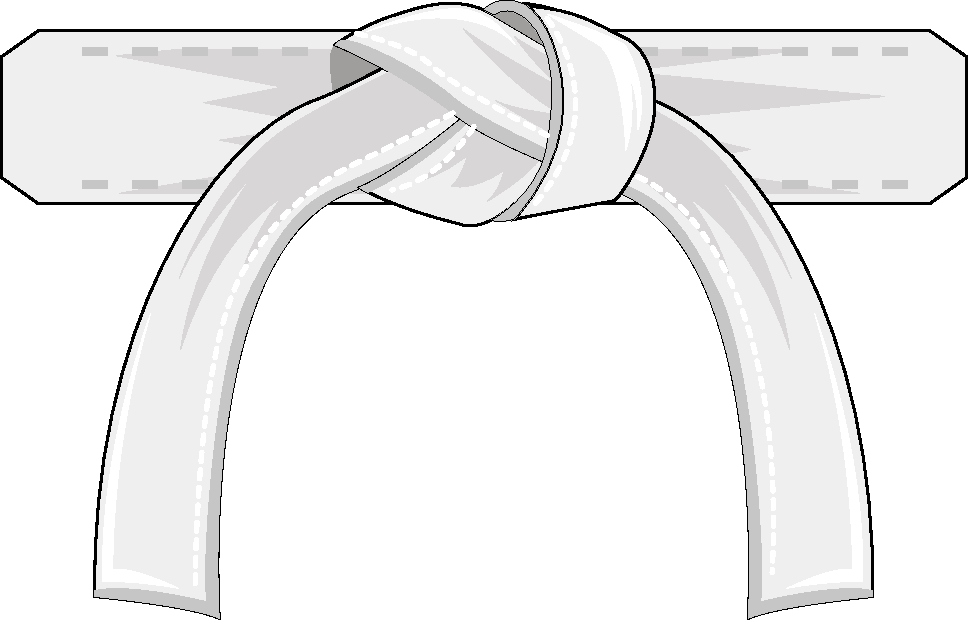
\includegraphics[height=14pt]{Gfx/gurte/whitebelt}}\\ \text{9.\,Kyu} & \raisebox{-4.2pt}{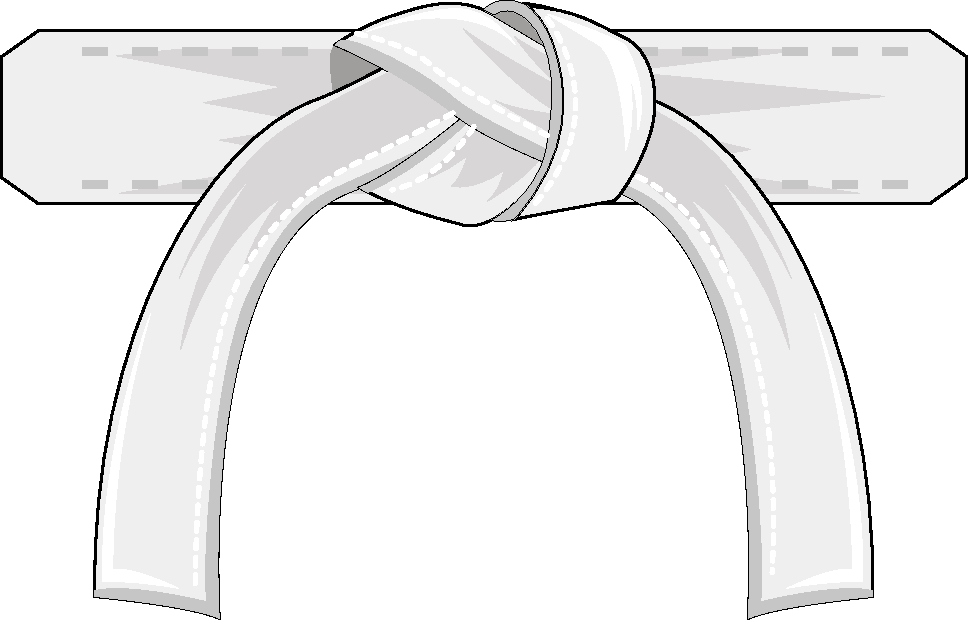
\includegraphics[height=14pt]{Gfx/gurte/whitebelt}}\\ \text{8.\,Kyu} & \raisebox{-4.2pt}{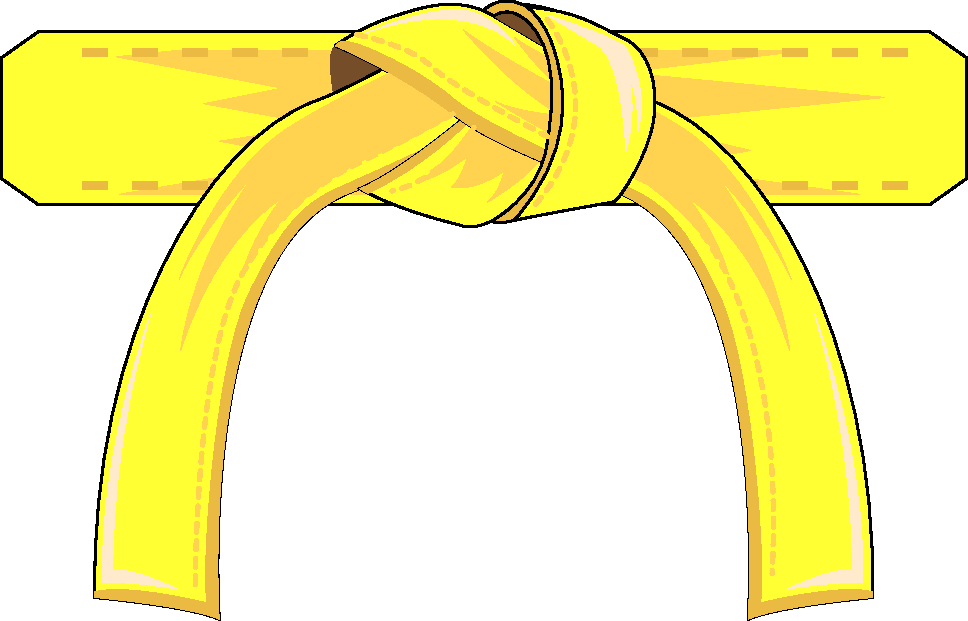
\includegraphics[height=14pt]{Gfx/gurte/yellowbelt}}\\ \text{7.\,Kyu}& \raisebox{-4.2pt}{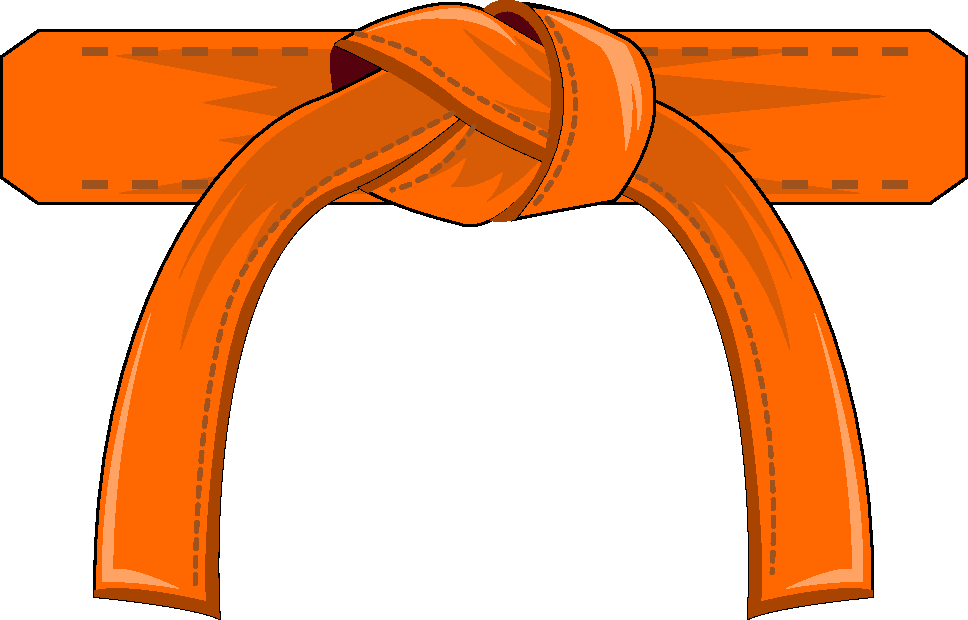
\includegraphics[height=14pt]{Gfx/gurte/orangebelt}}\end{array} \right\}\text{Unterstufe}$\quad$\left.\begin{array}{cl} \text{6.\,Kyu} & \raisebox{-4.2pt}{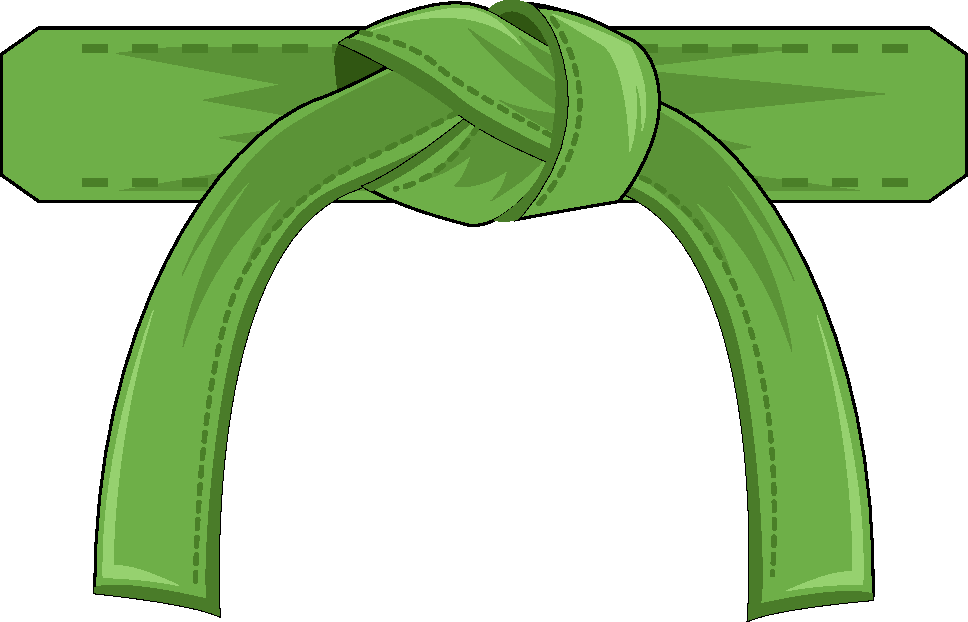
\includegraphics[height=14pt]{Gfx/gurte/greenbelt}} \\ \text{5.\,Kyu} & \raisebox{-4.2pt}{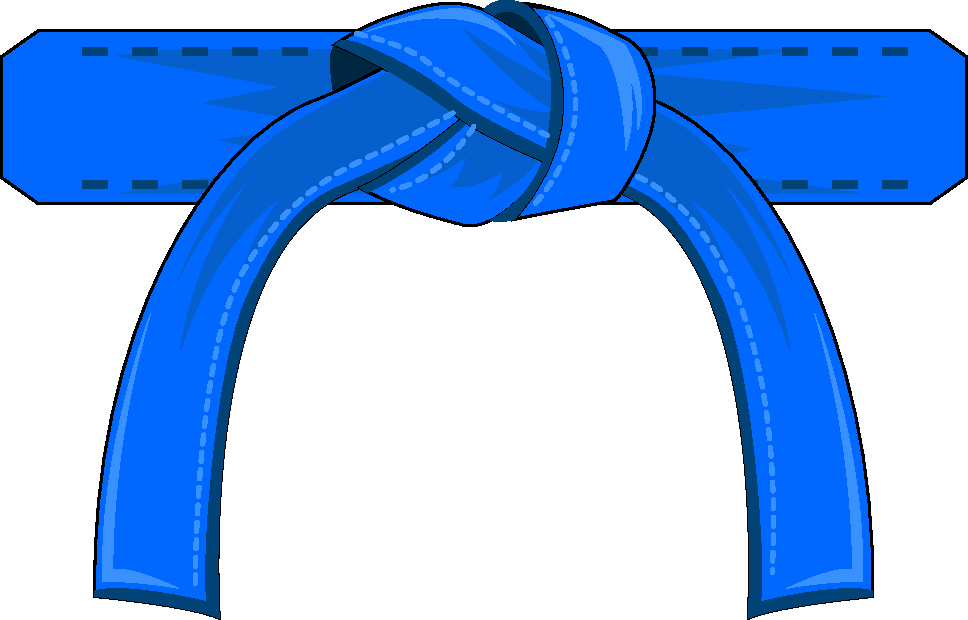
\includegraphics[height=14pt]{Gfx/gurte/bluebelt}}\\ \text{4.\,Kyu} & \raisebox{-4.2pt}{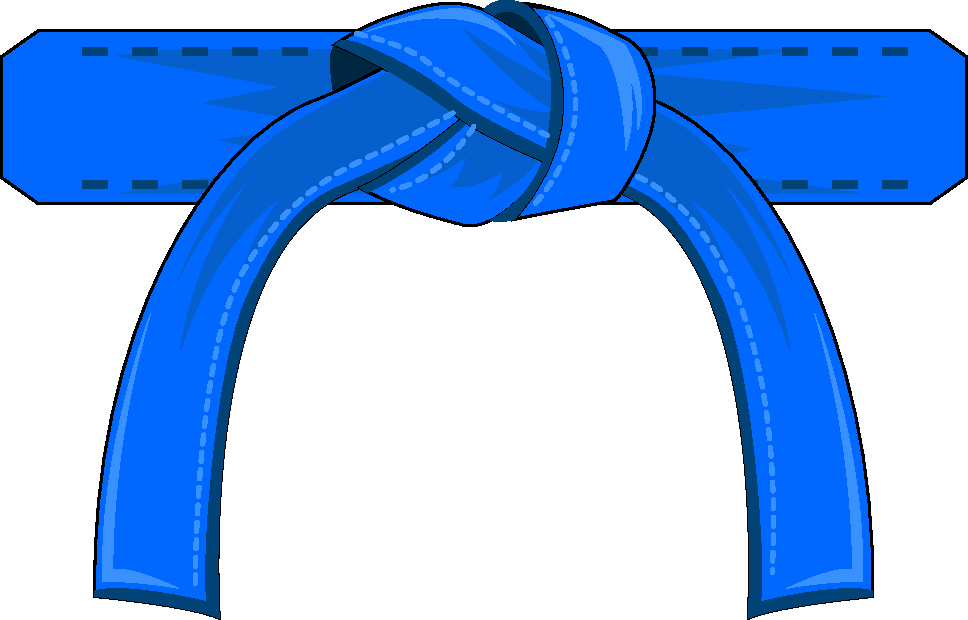
\includegraphics[height=14pt]{Gfx/gurte/bluebelt}}\end{array} \right\}\text{Mittelstufe}$\quad$\left.\begin{array}{cl} \text{3.\,Kyu} & \raisebox{-4.2pt}{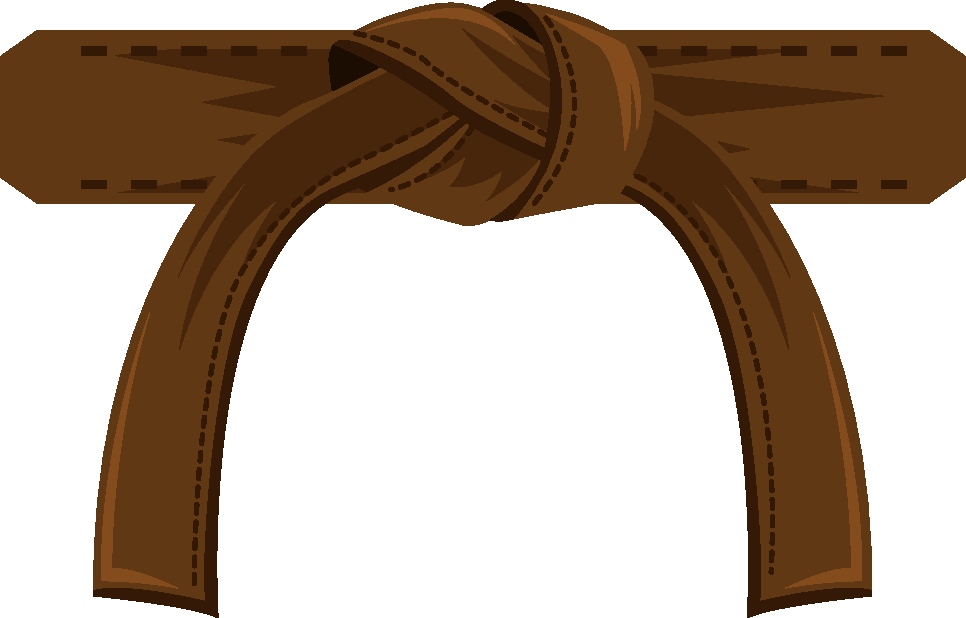
\includegraphics[height=14pt]{Gfx/gurte/brownbelt}}\\ \text{2.\,Kyu} & \raisebox{-4.2pt}{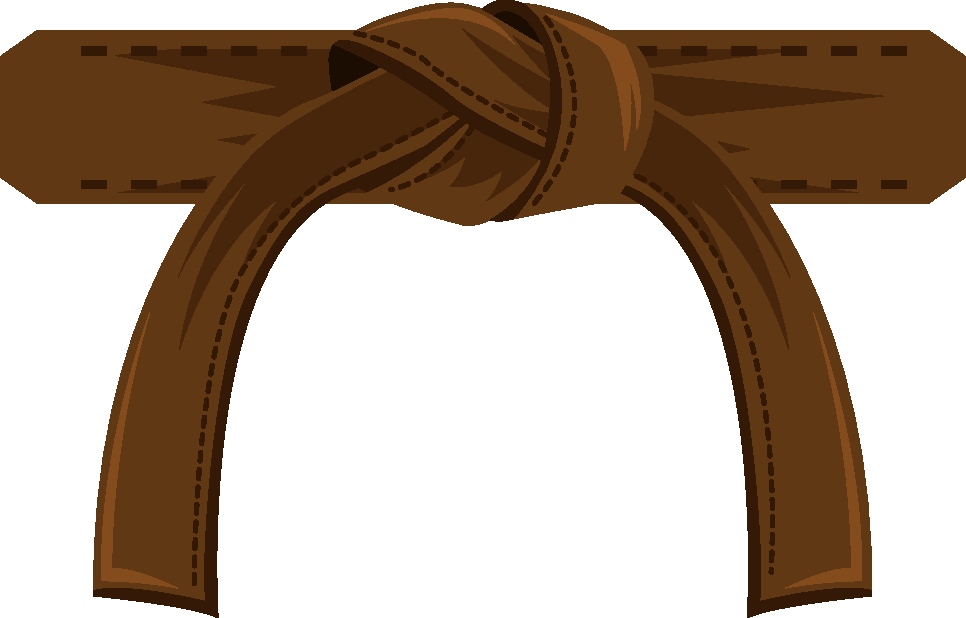
\includegraphics[height=14pt]{Gfx/gurte/brownbelt}} \\ \text{1.\,Kyu} & \raisebox{-4.2pt}{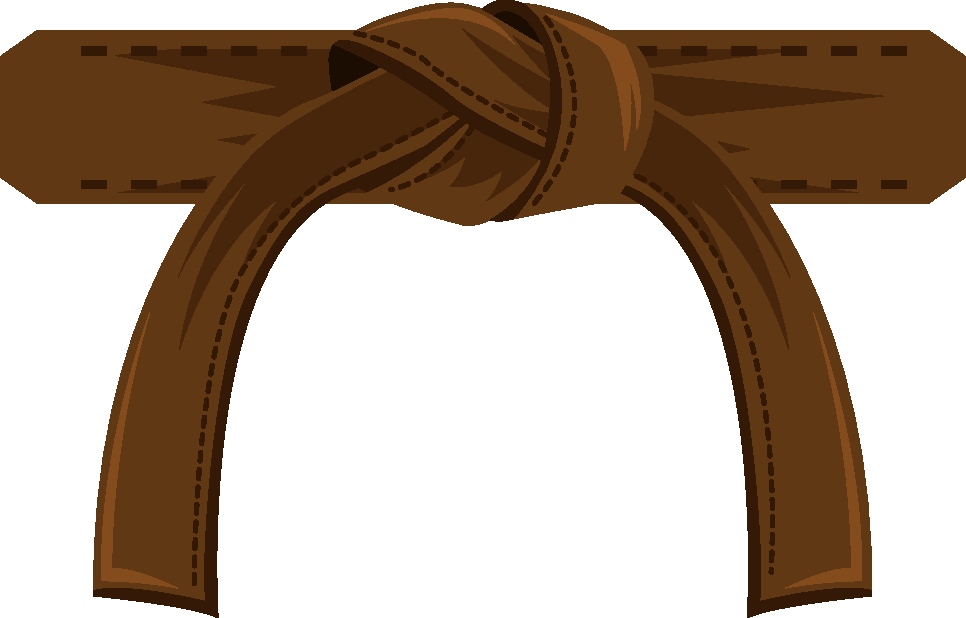
\includegraphics[height=14pt]{Gfx/gurte/brownbelt}}\end{array} \right\}\text{Oberstufe}$
		\end{center}
		
		Die Kyugrade werden meist in unserem Dojo von unseren Trainern, die auch eine Prüferlizenz haben, geprüft. Das jeweilige Prüfungsprogramm, sprich die zugrunde liegenden Techniken, Partnerformen, Kata sowie Kata-Bunkai, werden auf den späteren Trainingskarten aufgelistet.\\
		
		Prüfungen finden meist 2\textit{x}\,pro Jahr statt und die wöchentlichen Trainingseinheiten legen den Schwerpunkt jeweils ca. 8 Wochen vor der Prüfung auf die für die jeweiligen Prüflinge notwendigen Prüfungsinhalte. Je nach Anforderung werden dann innerhalb des Trainings entsprechende Gruppen gebildet, um eine gezielte Vorbereitung zu ermöglichen.\\
		
		\textit{Besonderheiten unseres Dojo:} Der Prüfungsinhalt zum 1.\,Kyu umfasst, zusätzlich zum eigentlichen Programm, ebenfalls die Inhalte der ebenfalls an diesem Tag stattfindenden Prüfungen - wenn zum Beispiel zur Prüfung zum 1.\,Kyu zwei Karateka angemeldet sind, sowie jeweils ein Karateka zum 9.,\,5.\,und 7.\,Kyu, so gehen die beiden zuerst genannten die jeweiligen Prüfungsprogramme der anderen ebenfalls mit - mit Ausnahme von Partnerformen und Kata-Bunkai. Findet an diesem Tag keine andere Prüfung statt, werden weitere Prüfinhalte im Vorfeld abgesprochen.
	}
\end{center}\null\vfill\null
%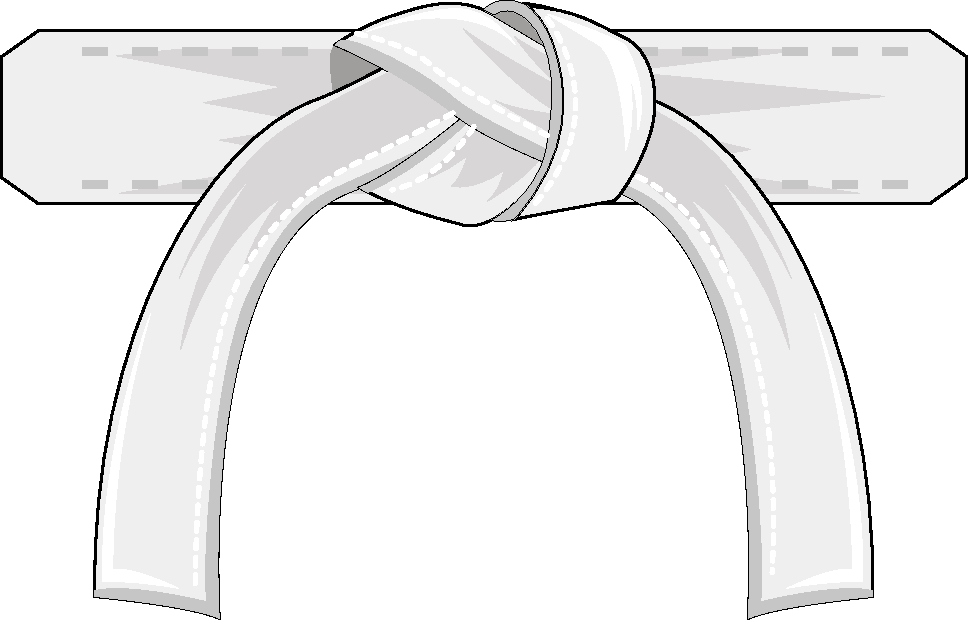
\includegraphics[height=\textheight]{Gfx/gurte/whitebelt}
\end{tcolorbox}
%%------------------------------------------------------------------------------
\clearpage
\pagebreak
%%------------------------------------------------------------------------------
\setcounter{num}{0}
\setcounter{numz}{0}
\setlength{\tabcolsep}{3pt}		
\begin{tcolorbox}[width=\textwidth,height=\textheight,right=12pt,left=12pt,colframe=GKD,colback=white,fonttitle=\bfseries,coltitle=white,title={Allgemeines:\indent Grundsätzliche Bewerungshorizonte für Unterstufe, Mittelstufe und Oberstufe}]
	\null\vfill\null
	\begin{center}
		\parbox{\textwidth-2\tabcolsep}{Es werden alle 6 Stände \& Techniken am Stück durchgeführt, in der Art, das immer der jeweils vordere Arm blockt (bzw. für die Fußtechniken der vordere Fuß kickt) und alle Standwechsel lediglich über den vorderen Fuß erfolgen. Als erste Übungsform wird nur der Block ausgeführt, als erste Steigerungsform wird der Konter hinzugenommen, als letzte Steigerung dann \mbox{Block \(\Rightarrow\)\,Kick \(\Rightarrow\)\,Konter.}}
	\end{center}\null\vfill\null
\end{tcolorbox}
%%------------------------------------------------------------------------------
\clearpage
\pagebreak
%%------------------------------------------------------------------------------